%$Header: /cvsroot/esrg/sfesrg/esrgpcpj/hyreach/doc/hyreachm/hyreachm.tex,v 1.16 2002/01/30 00:51:04 dtashley Exp $
%
%Standard packages included.
\documentclass[letterpaper,11pt,twoside,titlepage]{article}
\pagestyle{headings}
\usepackage{amsmath}
\usepackage{amsfonts}
\usepackage{amssymb}
\usepackage[ansinew]{inputenc}
\usepackage[OT1]{fontenc}
\usepackage{makeidx}
\usepackage{graphicx}
%

%Standard preamable.
\makeindex
%
%User-defined environments.
%$Header: /cvsroot/esrg/sfesrg/esrgpcpj/doc/engman01/general/newenvs.tex,v 1.2 2002/06/24 06:39:55 dtashley Exp $
%
%%%%%%%%%%%%%%%%%%%%%%%%%%%%%%%%%%%%%%%%%%%%%%%%%%%%%%%%%%%%%%%%%%%%%%%%%%%%%
%% GLOSSARY OF TERMS
%%%%%%%%%%%%%%%%%%%%%%%%%%%%%%%%%%%%%%%%%%%%%%%%%%%%%%%%%%%%%%%%%%%%%%%%%%%%%
%
%The following environment is for the glossary of terms.
\newenvironment{glossaryenum}{\begin{list}
               {}{\setlength{\labelwidth}{0mm}
                  \setlength{\leftmargin}{4mm}
                  \setlength{\itemindent}{-4mm}
                  \setlength{\parsep}{0.85mm}}}
               {\end{list}}
%
%%%%%%%%%%%%%%%%%%%%%%%%%%%%%%%%%%%%%%%%%%%%%%%%%%%%%%%%%%%%%%%%%%%%%%%%%%%%%%%%%%%%%%%%%%
%%%%%%%%%%%%%%%%%%%%%%%%%%%%%%%%%%%%%%%%%%%%%%%%%%%%%%%%%%%%%%%%%%%%%%%%%%%%%%%%%%%%%%%%%%
%%%%%%%%%%%%%%%%%%%%%%%%%%%%%%%%%%%%%%%%%%%%%%%%%%%%%%%%%%%%%%%%%%%%%%%%%%%%%%%%%%%%%%%%%%
%
%$Log: newenvs.tex,v $
%Revision 1.2  2002/06/24 06:39:55  dtashley
%Minor formatting change in log.
%
%Revision 1.1  2002/06/24 06:39:22  dtashley
%Initial checkin.
%
%End of file NEWENVS.TEX


\begin{document}

%The name of the tool is still in a state of flux.  Let's make this
%a command.
\newcommand{\swname}{HyReach}

%The version of the software may change.  Let's localize that.
\newcommand{\swversion}{1.0}

%The order and number of authors may change.  Let's assume for now
%that there will be only two authors.  I do not know who should be
%listed first.  Swapping the strings below should change everything
%in the document.
\newcommand{\authors}{David T. Ashley and Feng Lin}
\newcommand{\authorone}{David T. Ashley}
\newcommand{\authortwo}{Feng Lin}

\title{\swname{} User's Manual}
\author{David T. Ashley and Feng Lin}
\date{2001-09-25}

%Make the title page of the document.
%$Header: /cvsroot/esrg/sfesrg/esrgpcpj/doc/engman01/general/tpage.tex,v 1.3 2002/06/24 20:49:15 dtashley Exp $

\thispagestyle{empty}
\vspace*{0.0cm}
\begin{flushright}
\Huge\bfseries
\tsname{} Version \tsversion{} Engineering Manual
\end{flushright}
\vspace{0.0cm}
\noindent\rule{\textwidth}{2pt}
\begin{flushright}
\Large\bfseries
This manual covers administrative and technical matters
related to the production and release of
\emph{The \tsname{} Version \tsversion{}}, and is
intended for those who must build the 
tool set from source code, modify the tool set,
contribute to the tool set, or release the tool set.
\end{flushright}
\vfill
\begin{flushright}
\begin{small}
\authors{}
\end{small}
\end{flushright}
\vspace{0.2cm}
\begin{flushright}
\begin{small}
Document compiled from \LaTeX{} source code on \today .
\end{small}
\end{flushright}
\vspace*{0.0cm}

\pagebreak
\thispagestyle{empty}
\begin{small}
  \noindent Copyright \copyright 2002 \authors{}.
\end{small}

\vfill

%%%%%%%%%%%%%%%%%%%%%%%%%%%%%%%%%%%%%%%%%%%%%%%%%%%%%%%%%%%%%%%%%%%%%%%%%%
\noindent\begin{figure}[!b]
\noindent\rule[-0.25in]{\textwidth}{1pt}
\begin{tiny}
\begin{verbatim}
$RCSfile: tpage.tex,v $
$Source: /cvsroot/esrg/sfesrg/esrgpcpj/doc/engman01/general/tpage.tex,v $
$Revision: 1.3 $
$Author: dtashley $
$Date: 2002/06/24 20:49:15 $
\end{verbatim}
\end{tiny}
\noindent\rule[0.25in]{\textwidth}{1pt}
\end{figure}
%%%%%%%%%%%%%%%%%%%%%%%%%%%%%%%%%%%%%%%%%%%%%%%%%%%%%%%%%%%%%%%%%%%%%%%%%%
%
%$Log: tpage.tex,v $
%Revision 1.3  2002/06/24 20:49:15  dtashley
%Edits.
%
%Revision 1.2  2002/06/24 06:38:24  dtashley
%Minor log formattting change.
%
%Revision 1.1  2002/06/24 06:38:00  dtashley
%Initial checkin.
%
%End of TPAGE.TEX

\clearpage

\raggedbottom
\tableofcontents
\clearpage

\listoffigures
%\pagebreak

\listoftables

%SOSP0: Overview, Scope, And Purpose
\clearpage{}
%$Header: /cvsroot/esrg/sfesrg/esrgpcpj/hyreach/doc/hyreachm/s_osp0/s_osp0.tex,v 1.6 2002/01/29 17:04:00 dtashley Exp $
%
\section{Overview, Scope, And Purpose}
\label{sosp0}

This document describes the \swname{} software, Version \swversion{}.  
\swname{} is a software 
program to determine the reachability of certain states of timed automata models 
under a very restricted modeling framework.  The software was specifically crafted 
to solve the interrupt latency compatibility problem for practical embedded systems.

The mnemonic behind the name \swname{} is \emph{hy}brid system 
\emph{reach}ability.  \swname{} is not 
related in any way to the hybrid system tool from Stanford, \emph{HyTech}.

Although the source code for \swname{} is very portable (primarily because it does 
not include a graphical interface), at the present time only an executable for Windows 
platforms is provided.

Section \ref{sinv0} describes the invocation of the software, 
including command-line parameters 
and output.

Section \ref{smfs0} describes the modeling framework supported. 
To achieve good performance on 
models of practical size, a very restricted modeling framework is supported.

Section \ref{siff0} describes the input file format required by \swname{}.  
The input file is a 
text file which specifies the system to be analyzed for reachability.

Section \ref{srae0} supplies the details of the reachability algorithm employed.

Section \ref{ssym0} describes the modeling of practical systems in idioms 
that \swname{} can accept.

Section \ref{siop0} describes the design of \swname{}---primarily 
the optimizations for speed.

Section \ref{spbd0} describes the benchmarking of \swname{}.  \swname{} is benchmarked 
against UPPAAL (a verification tool with a similar philosophy but with far more 
verification capability).  The verification time of \swname{} is extrapolated with 
respect to the number of automatons and their number of states.

Section \ref{sack0} contains acknowledgements to the organizations and individuals
who have assisted us in this work.

Section \ref{sglo0} provides a glossary of terms, since the nomenclature we use
may in some cases be non-standard.

Section \ref{sglm0} provides a glossary of mathematical notation and symbols.

An index is also provided at the end of the document.


%%%%%%%%%%%%%%%%%%%%%%%%%%%%%%%%%%%%%%%%%%%%%%%%%%%%%%%%%%%%%%%%%%%%%%%%%%
\noindent\begin{figure}[!b]
\noindent\rule[-0.25in]{\textwidth}{1pt}
\begin{tiny}
\begin{verbatim}
$RCSfile: s_osp0.tex,v $
$Source: /cvsroot/esrg/sfesrg/esrgpcpj/hyreach/doc/hyreachm/s_osp0/s_osp0.tex,v $
$Revision: 1.6 $
$Author: dtashley $
$Date: 2002/01/29 17:04:00 $
\end{verbatim}
\end{tiny}
\noindent\rule[0.25in]{\textwidth}{1pt}
\end{figure}
%%%%%%%%%%%%%%%%%%%%%%%%%%%%%%%%%%%%%%%%%%%%%%%%%%%%%%%%%%%%%%%%%%%%%%%%%%
%$Log: s_osp0.tex,v $
%Revision 1.6  2002/01/29 17:04:00  dtashley
%Version control info added, and minor edits.
%
%Revision 1.5  2001/10/31 04:31:37  dtashley
%Nightly safety checkin.
%
%Revision 1.4  2001/10/12 22:32:30  dtashley
%Substantial edits.
%
%Revision 1.3  2001/10/10 02:09:07  dtashley
%Edits.
%
%Revision 1.2  2001/09/26 04:51:13  dtashley
%Edits.
%
%Revision 1.1  2001/09/26 02:31:14  dtashley
%Initial checkin, and some edits of main TEX file.
%
%End of S_OSP0.TEX.


%SINV0: Invocation Of The Software
\clearpage{}
%$Header: /cvsroot/esrg/sfesrg/esrgpcpj/hyreach/doc/hyreachm/s_inv0/s_inv0.tex,v 1.6 2002/01/30 00:51:04 dtashley Exp $
%
\section{Invocation Of The Software}
\label{sinv0}

\swname{} is an ordinary Win32 console application, produced using Microsoft 
Visual C++ Version 6.0.  When \swname{} is invoked, it undertakes the following actions:

\begin{itemize}
\item \index{command-line parameters}Command-line 
      parameters are parsed.  Fatal errors are possible if 
      the command-line parameters are ill-formatted.
\item The input file (which specifies the model to verify) is parsed.  
      Fatal errors are possible if the model file is ill-formatted.
\item 
      \index{model design rules}Design-rule 
      checks are applied to the model specified.
      Fatal errors are possible if the model specified violates the design 
      rules.
\item A reachability algorithm is applied to determine if any of the configurations
      marked as illegal in the model are reachable.  When invoked and
      unless stopped by the user, \swname{} will do 
      one of the following:
      
      \begin{itemize}
      \item Verify that no illegal state is reachable.
      \item Determine that an illegal configuration is reachable, and indicate how, 
            starting from the initial configurations, an illegal configuration can be reached.
      \item Terminate abnormally without a reachability determination because 
            not enough computer resources (memory) are available to perform 
            the verification.
      \end{itemize}
\end{itemize}

Once invoked, \swname{} can be terminated before it completes normally in
two ways:

\begin{itemize}
\item Using the CTRL-C or CTRL-BREAK key combinations while the console
      window in which \swname{} is running has the focus.
\item Using the CTRL-ALT-DELETE key combination to obtain a list of applications
      or processes, and then electing to terminte \swname{}.
\end{itemize}

Of the two termination alternatives, the first is preferred, as it works using
the 'C' runtime library and is a gentler type of termination.


\subsection{Invocation Format}
%Subsection Tag: SINF0
\label{sinv0:sinf0}

The general invocation format is: \\

\texttt{hyreach option\_1 option\_2 \ldots option\_N} \\

\noindent{}where the options are any of the options 
described in Section \ref{sinv0:sclo0}.  Note that 
one of the options (the \texttt{-mf}, or \emph{model file} 
option) is not truly optional, as \swname{} will not 
do any useful work without it.

Note that each option consists of an option flag
(``\texttt{-mf}'', for example) followed by zero
or more option parameters.  The number of required
option parameters is fixed for each option.

Options may always appear in any order, but may not
appear twice.


%%%%%%%%%%%%%%%%%%%%%%%%%%%%%%%%%%%%%%%%%%%%%%%%%%%%%%%%%%%%%%%%%%%%%%%%%%%%%%%
%%%%%%%%%%%%%%%%%%%%%%%%%%%%%%%%%%%%%%%%%%%%%%%%%%%%%%%%%%%%%%%%%%%%%%%%%%%%%%%
%%%%%%%%%%%%%%%%%%%%%%%%%%%%%%%%%%%%%%%%%%%%%%%%%%%%%%%%%%%%%%%%%%%%%%%%%%%%%%%
\subsection{Command-Line Options}
%Subsection Tag: SCLO0
\label{sinv0:sclo0}

This section describes the command-line options that may be used to modify the 
behavior of \swname{}.

\subsubsection{-mf Command-Line Option (1 Option Parameter)}
The \index{-mf@\texttt{-mf}}\texttt{-mf} (``model file'') specifies to 
\swname{} the name of the model file to be used (the format of
the model file is described in Section \ref{siff0}).
\swname{} performs no processing or interpretation of the string
supplied, so the filename specified may be any filename accepted
by the underlying operating system.

If the model file name specified contains spaces, the name must be
surrounded by quotes.\footnote{Strictly speaking, this isn't always true.
The issue is how \swname{} receives its arguments (the \texttt{argv[]} 
array).  If a file name containing spaces is specified from within a DOS
box, the quotes prevent the DOS command interpreter from interpreting the
file name as multiple parameters and breaking it up.  However, if a
scripting language such a Tcl is used, it may not be necessary to quote
such a file name (and in fact it may cause errors) because the 
spawning mechanisms (the \texttt{exec} command in Tcl for example) 
bypass the DOS command interpeter.}

\subsubsection{-ch Command-Line Option (No Option Parameters)}
The \index{-ch@\texttt{-ch}}\texttt{-ch} (``convex hull'') command-line 
option causes \swname{} to transform unions of convex zones to
the minimal convex zone (the \index{convex hull}convex hull) 
that will enclose the union.  
(Note that the convex hull is at least as large as union.)
Since these 
unions are used to represent the subset of $\mathbb{R}^N$ that 
clock variables may be in, any states that are reachable using the exact
representation (the union) are also reachable using the convex hull 
approximation; but the converse is not true.  Thus:

\begin{itemize}
\item A result of ``no illegal configurations reachable'' when the 
      \texttt{-ch} option is used implies that the configurations will also
      not be reachable when the more exact representation is used.
\item A result of ``illegal configurations reachable'' when the 
      \texttt{-ch} option is used does not necessarily imply that 
      illegal configurations will be reachable when the more exact
      representation is used.
\end{itemize}

Thus, with respect to the safeness of systems, the \texttt{-ch}
option cannot lead to a false determination of \emph{safe}, but
can lead to a false determination of \emph{unsafe}.

\subsubsection{-q Command-Line Option (No Option Parameters)}
The \index{-q@\texttt{-q}}\texttt{-q} (``quiet'') command-line option causes \swname{}
to produce a minimal amount of output.  This option is approximately opposite
to the \texttt{-d} (debug level) and \texttt{-v} (verbose)
command-line options.

\subsubsection{-v Command-Line Option (No Option Parameters)}
The \index{-v@\texttt{-v}}\texttt{-v} (``verbose'') command-line option causes 
\swname{} to produce more than the normal 
amount of output.  The output is of an informational nature, and not 
designed to assist in debugging.

\subsubsection{-d Command-Line Option (2 Option Parameters)}
The \index{-d@\texttt{-d}}\texttt{-d <debug\_level> <debug\_file\_name>} (``debug'') 
command-line option causes 
\swname{} to produce information 
useful in debugging.  The \texttt{debug\_level}
integral parameter to this option 
must be one of the numerical parameters described in Table 
\ref{tbl:sinv0:sclo0:01}.

\begin{table}
\begin{center}
\begin{tabular}{|c|l|}
\hline
\texttt{-d} Option Value & Interpretation \\
\hline
\hline
0 (default) & No debugging information is produced.  Although a              \\
            & file name must be specified because of the syntax              \\
            & of the option, no debug file will be produced.                 \\
\hline
1           & Information is provided to trace what the program              \\
            & is doing and when.  Certain abstract information,              \\
            & such as size or complexity measures for data                   \\
            & structures or timing information will be produced.             \\
\hline
2           & Abstract data structure information will be                    \\
            & produced.  Generally by \emph{abstract} we mean that           \\
            & the interpretation of data structures (the                     \\
            & represented polytopes, for example) will be                    \\
            & produced, but the implementation details of data               \\
            & structures (pointer values, bitfield values, etc)              \\
            & will not be produced.                                          \\
\hline
3           & Detailed data structure information (including                 \\
            & implementation details) will be produced.                      \\
\hline
4           & All available information will be produced.                    \\
\hline
\end{tabular}
\end{center}
\caption{\texttt{-d} Option Parameters And Their Interpretation}
\label{tbl:sinv0:sclo0:01}
\end{table}

The \texttt{debug\_file\_name} parameter must be a file that can be
opened by the operating system.  At the higher debug levels, operation
of \swname{} will be slowed substantially, and the debug information
file may become quite large.  Note also that \swname{} can be compiled
without debug support (for the sake of speed), in which case 
the \texttt{-d} option will not be allowed.

%%%%%%%%%%%%%%%%%%%%%%%%%%%%%%%%%%%%%%%%%%%%%%%%%%%%%%%%%%%%%%%%%%%%%%%%%%
\noindent\begin{figure}[!b]
\noindent\rule[-0.25in]{\textwidth}{1pt}
\begin{tiny}
\begin{verbatim}
$RCSfile: s_inv0.tex,v $
$Source: /cvsroot/esrg/sfesrg/esrgpcpj/hyreach/doc/hyreachm/s_inv0/s_inv0.tex,v $
$Revision: 1.6 $
$Author: dtashley $
$Date: 2002/01/30 00:51:04 $
\end{verbatim}
\end{tiny}
\noindent\rule[0.25in]{\textwidth}{1pt}
\end{figure}
%%%%%%%%%%%%%%%%%%%%%%%%%%%%%%%%%%%%%%%%%%%%%%%%%%%%%%%%%%%%%%%%%%%%%%%%%%
%$Log: s_inv0.tex,v $
%Revision 1.6  2002/01/30 00:51:04  dtashley
%Nightly safety checkin.
%
%Revision 1.5  2002/01/29 17:04:00  dtashley
%Version control info added, and minor edits.
%
%Revision 1.4  2001/10/12 22:32:30  dtashley
%Substantial edits.
%
%Revision 1.3  2001/10/10 02:09:07  dtashley
%Edits.
%
%Revision 1.2  2001/09/26 04:51:13  dtashley
%Edits.
%
%Revision 1.1  2001/09/26 02:31:14  dtashley
%Initial checkin, and some edits of main TEX file.
%
%End of S_INV0.TEX.


%SMFS0: Modeling Framework Supported
\clearpage{}
%$Header: /cvsroot/esrg/sfesrg/esrgpcpj/hyreach/doc/hyreachm/s_mfs0/s_mfs0.tex,v 1.6 2002/01/29 17:04:00 dtashley Exp $
%
%%%%%%%%%%%%%%%%%%%%%%%%%%%%%%%%%%%%%%%%%%%%%%%%%%%%%%%%%%%%%%%%%%%%%%%%%%%%%%%
%%%%%%%%%%%%%%%%%%%%%%%%%%%%%%%%%%%%%%%%%%%%%%%%%%%%%%%%%%%%%%%%%%%%%%%%%%%%%%%
%%%%%%%%%%%%%%%%%%%%%%%%%%%%%%%%%%%%%%%%%%%%%%%%%%%%%%%%%%%%%%%%%%%%%%%%%%%%%%%
\section{Modeling Framework Supported}
%Section Tag: MFS0.
\label{smfs0}

The modeling framework of \swname{} has been optimized for the 
computational efficiency of checking reachability properties
of a timing model of the interrupt subsystem of a software load.
This has two consequences:

\begin{itemize}
\item The modeling framework is severely constrained; i.e. all unnecessary
      expressiveness has been removed from the framework.
\item The modeling framework contains novel features (such as 
      the explicit definition of configuration equivalence classes) which are
	  not strictly necessary but which are a modeling convenience for the
	  particular category of problem that \swname{} was designed to address.
\end{itemize}

The modeling framework used is very close to that presented in 
\cite{bib:p:theoryofta:alurdill90}, with restrictions.  In this section,
we describe the modeling framework and the restrictions.


%%%%%%%%%%%%%%%%%%%%%%%%%%%%%%%%%%%%%%%%%%%%%%%%%%%%%%%%%%%%%%%%%%%%%%%%%%%%%%%
%%%%%%%%%%%%%%%%%%%%%%%%%%%%%%%%%%%%%%%%%%%%%%%%%%%%%%%%%%%%%%%%%%%%%%%%%%%%%%%
%%%%%%%%%%%%%%%%%%%%%%%%%%%%%%%%%%%%%%%%%%%%%%%%%%%%%%%%%%%%%%%%%%%%%%%%%%%%%%%
\subsection{Nomenclature}
%Subsection Tag: NMC0.
\label{smfs0:snmc0}

We adopt a nomenclature closer to that used
in \cite{bib:p:hybridsysintlat:lin90} than in \cite{bib:p:theoryofta:alurdill90}.
In most cases, terms are explained in more detail in Section \ref{sglo0}.

Generally, we seek to model the components which affect interrupt latency 
compatibility (software components such as critical sections and interrupt
service routines; as well as hardware components such as interrupt priority
resolution logic and communication peripherals) in a hybrid system framework.
In describing a system as \emph{hybrid}, we mean that its state vector is a mixture
of both discrete state and continuous state.

However, the systems we wish to evaluate for the absence or presence of certain
properties can be described without the full expressiveness
inherent in the notion of a hybrid system.  For example, in the software systems
of interest to us, the only continuous quantity of interest is usually time, and
thus all continuous variables in the system evolve at rate $\dot{x}_n = 1$ and it
isn't necessary to consider general differential equations.  The simplified framework
in which we model practical systems is the \emph{timed automata} framework as described
in \cite{bib:p:theoryofta:alurdill90}.


%%%%%%%%%%%%%%%%%%%%%%%%%%%%%%%%%%%%%%%%%%%%%%%%%%%%%%%%%%%%%%%%%%%%%%%%%%%%%%%
%%%%%%%%%%%%%%%%%%%%%%%%%%%%%%%%%%%%%%%%%%%%%%%%%%%%%%%%%%%%%%%%%%%%%%%%%%%%%%%
%%%%%%%%%%%%%%%%%%%%%%%%%%%%%%%%%%%%%%%%%%%%%%%%%%%%%%%%%%%%%%%%%%%%%%%%%%%%%%%
\subsection{Collection Of Cooperating EHMs}
%Subsection Tag: CCE0.
\label{smfs0:scce0}

The modeling framework accepted by \swname{} involves specifying a collection
of cooperating EHMs, $\{ \lambda_1, \ldots{}, \lambda_N \}$.  Each EHM $\lambda_i$
has 
two components to its state:

\begin{itemize}
\item A discrete component, which we call the \emph{configuration}.
\item Zero or more \emph{clocks}, $C_{ij}$, which can only assume
      non-negative integer values (Section \ref{smfs0:srit0}).
\end{itemize}

It is possible through a well-defined composition operation to combine all
EHMs into a CHM, which we denote $\Lambda$.  The CHM has the same design rules
as an EHM, but embodies the state space of all EHMs acting concurrently.

%%%%%%%%%%%%%%%%%%%%%%%%%%%%%%%%%%%%%%%%%%%%%%%%%%%%%%%%%%%%%%%%%%%%%%%%%%%%%%%
%%%%%%%%%%%%%%%%%%%%%%%%%%%%%%%%%%%%%%%%%%%%%%%%%%%%%%%%%%%%%%%%%%%%%%%%%%%%%%%
%%%%%%%%%%%%%%%%%%%%%%%%%%%%%%%%%%%%%%%%%%%%%%%%%%%%%%%%%%%%%%%%%%%%%%%%%%%%%%%
\subsection{Initial Conditions}
%Subsection Tag: ICO0.
\label{smfs0:sico0}

For modeling, each $\lambda_i$ has a unique initial configuration, which in figures we 
denote with a wedge (Fig. \ref{fig:smfs0:sico0:00}).  It is also assumed that 
every clock owned by every EHM starts with the value of 0.

\begin{figure}
\centering
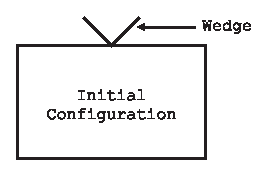
\includegraphics[height=1.0in]{s_mfs0/figini01.eps}
\caption{Initial Configuration Of EHM Depicted Using Wedge}
\label{fig:smfs0:sico0:00}
\end{figure}

For most practical models, the initial conditions described are adequate.
However, if different initial conditions are required, they can be 
created by 


%%%%%%%%%%%%%%%%%%%%%%%%%%%%%%%%%%%%%%%%%%%%%%%%%%%%%%%%%%%%%%%%%%%%%%%%%%%%%%%
%%%%%%%%%%%%%%%%%%%%%%%%%%%%%%%%%%%%%%%%%%%%%%%%%%%%%%%%%%%%%%%%%%%%%%%%%%%%%%%
%%%%%%%%%%%%%%%%%%%%%%%%%%%%%%%%%%%%%%%%%%%%%%%%%%%%%%%%%%%%%%%%%%%%%%%%%%%%%%%
\subsection{Restriction To Integer Time}
%Subsection Tag: RIT0.
\label{smfs0:srit0}


%%%%%%%%%%%%%%%%%%%%%%%%%%%%%%%%%%%%%%%%%%%%%%%%%%%%%%%%%%%%%%%%%%%%%%%%%%%%%%%
%%%%%%%%%%%%%%%%%%%%%%%%%%%%%%%%%%%%%%%%%%%%%%%%%%%%%%%%%%%%%%%%%%%%%%%%%%%%%%%
%%%%%%%%%%%%%%%%%%%%%%%%%%%%%%%%%%%%%%%%%%%%%%%%%%%%%%%%%%%%%%%%%%%%%%%%%%%%%%%
\subsection{Restriction To $\geq$ And $<$}
%Subsection Tag: RGE0.
\label{smfs0:srge0}


%%%%%%%%%%%%%%%%%%%%%%%%%%%%%%%%%%%%%%%%%%%%%%%%%%%%%%%%%%%%%%%%%%%%%%%%%%%%%%%
%%%%%%%%%%%%%%%%%%%%%%%%%%%%%%%%%%%%%%%%%%%%%%%%%%%%%%%%%%%%%%%%%%%%%%%%%%%%%%%
%%%%%%%%%%%%%%%%%%%%%%%%%%%%%%%%%%%%%%%%%%%%%%%%%%%%%%%%%%%%%%%%%%%%%%%%%%%%%%%
\subsection{Guards And Invariants}
%Subsection Tag: GAI0.
\label{smfs0:sgai0}


%%%%%%%%%%%%%%%%%%%%%%%%%%%%%%%%%%%%%%%%%%%%%%%%%%%%%%%%%%%%%%%%%%%%%%%%%%%%%%%
%%%%%%%%%%%%%%%%%%%%%%%%%%%%%%%%%%%%%%%%%%%%%%%%%%%%%%%%%%%%%%%%%%%%%%%%%%%%%%%
%%%%%%%%%%%%%%%%%%%%%%%%%%%%%%%%%%%%%%%%%%%%%%%%%%%%%%%%%%%%%%%%%%%%%%%%%%%%%%%
\subsection{Strong Synchronization (Events)}
%Subsection Tag: SSY0.
\label{smfs0:sssy0}


%%%%%%%%%%%%%%%%%%%%%%%%%%%%%%%%%%%%%%%%%%%%%%%%%%%%%%%%%%%%%%%%%%%%%%%%%%%%%%%
%%%%%%%%%%%%%%%%%%%%%%%%%%%%%%%%%%%%%%%%%%%%%%%%%%%%%%%%%%%%%%%%%%%%%%%%%%%%%%%
%%%%%%%%%%%%%%%%%%%%%%%%%%%%%%%%%%%%%%%%%%%%%%%%%%%%%%%%%%%%%%%%%%%%%%%%%%%%%%%
\subsection{Weak Synchronization (Guards Dependent On Configuration)}
%Subsection Tag: WSY0.
\label{smfs0:swsy0}


%%%%%%%%%%%%%%%%%%%%%%%%%%%%%%%%%%%%%%%%%%%%%%%%%%%%%%%%%%%%%%%%%%%%%%%%%%%%%%%
%%%%%%%%%%%%%%%%%%%%%%%%%%%%%%%%%%%%%%%%%%%%%%%%%%%%%%%%%%%%%%%%%%%%%%%%%%%%%%%
%%%%%%%%%%%%%%%%%%%%%%%%%%%%%%%%%%%%%%%%%%%%%%%%%%%%%%%%%%%%%%%%%%%%%%%%%%%%%%%
\subsection{Legal Versus Illegal Configurations}
%Subsection Tag: LVI0.
\label{smfs0:slvi0}


%%%%%%%%%%%%%%%%%%%%%%%%%%%%%%%%%%%%%%%%%%%%%%%%%%%%%%%%%%%%%%%%%%%%%%%%%%%%%%%
%%%%%%%%%%%%%%%%%%%%%%%%%%%%%%%%%%%%%%%%%%%%%%%%%%%%%%%%%%%%%%%%%%%%%%%%%%%%%%%
%%%%%%%%%%%%%%%%%%%%%%%%%%%%%%%%%%%%%%%%%%%%%%%%%%%%%%%%%%%%%%%%%%%%%%%%%%%%%%%
\subsection{Modeling Features Explicitly Not Supported}
%Subsection Tag: MEN0.
\label{smfs0:smen0}


%%%%%%%%%%%%%%%%%%%%%%%%%%%%%%%%%%%%%%%%%%%%%%%%%%%%%%%%%%%%%%%%%%%%%%%%%%
\noindent\begin{figure}[!b]
\noindent\rule[-0.25in]{\textwidth}{1pt}
\begin{tiny}
\begin{verbatim}
$RCSfile: s_mfs0.tex,v $
$Source: /cvsroot/esrg/sfesrg/esrgpcpj/hyreach/doc/hyreachm/s_mfs0/s_mfs0.tex,v $
$Revision: 1.6 $
$Author: dtashley $
$Date: 2002/01/29 17:04:00 $
\end{verbatim}
\end{tiny}
\noindent\rule[0.25in]{\textwidth}{1pt}
\end{figure}
%%%%%%%%%%%%%%%%%%%%%%%%%%%%%%%%%%%%%%%%%%%%%%%%%%%%%%%%%%%%%%%%%%%%%%%%%%
%$Log: s_mfs0.tex,v $
%Revision 1.6  2002/01/29 17:04:00  dtashley
%Version control info added, and minor edits.
%
%Revision 1.5  2001/10/31 04:31:37  dtashley
%Nightly safety checkin.
%
%Revision 1.4  2001/10/03 03:15:19  dtashley
%Nightly checkin.
%
%Revision 1.3  2001/10/02 03:16:54  dtashley
%Final edits evening of 10/01/01.
%
%Revision 1.2  2001/09/26 04:51:13  dtashley
%Edits.
%
%Revision 1.1  2001/09/26 02:31:14  dtashley
%Initial checkin, and some edits of main TEX file.
%
%End of S_MFS0.TEX.


%SIFF0: Input File Format
\clearpage{}
%$Header: /cvsroot/esrg/sfesrg/esrgpcpj/hyreach/doc/hyreachm/s_iff0/s_iff0.tex,v 1.4 2002/01/29 17:04:00 dtashley Exp $
%
\section{Input File Format}
\label{siff0}

\swname{} accepts a model input file which specifies the model 
to be verified for reachability properties.  This section of the
document specifies the format of this file.


%%%%%%%%%%%%%%%%%%%%%%%%%%%%%%%%%%%%%%%%%%%%%%%%%%%%%%%%%%%%%%%%%%%%%%%%%%%%%%%
%%%%%%%%%%%%%%%%%%%%%%%%%%%%%%%%%%%%%%%%%%%%%%%%%%%%%%%%%%%%%%%%%%%%%%%%%%%%%%%
%%%%%%%%%%%%%%%%%%%%%%%%%%%%%%%%%%%%%%%%%%%%%%%%%%%%%%%%%%%%%%%%%%%%%%%%%%%%%%%
\subsection{Overview And Essential Characteristics Of The Model Input File Format}
%Subsection Tag: OEC0
\label{siff0:soec0}

The model input file is an ASCII text file with the following characteristics.

\begin{enumerate}
\item The file is a plain ASCII text file rather than a binary file.
      This means the file can be prepared using an ordinary text editor, a 
      \texttt{.BAT} file, a script, etc.
\item The file is token- rather than record-oriented.  
      This means the file has a relatively free aesthetic format and can be 
      formatted to suit the tastes of the preparer.
\item Keywords and variables are case-sensitive.  
      \emph{Catsanddogs} is different than \emph{CatsAndDogs}.
\end{enumerate}

The remainder of the this section (Section \ref{siff0})
describes the format, and finally concludes with an example.


%%%%%%%%%%%%%%%%%%%%%%%%%%%%%%%%%%%%%%%%%%%%%%%%%%%%%%%%%%%%%%%%%%%%%%%%%%%%%%%
%%%%%%%%%%%%%%%%%%%%%%%%%%%%%%%%%%%%%%%%%%%%%%%%%%%%%%%%%%%%%%%%%%%%%%%%%%%%%%%
%%%%%%%%%%%%%%%%%%%%%%%%%%%%%%%%%%%%%%%%%%%%%%%%%%%%%%%%%%%%%%%%%%%%%%%%%%%%%%%
\subsection{Allowable Character Set}
%Subsection Tag: ACS0
\label{siff0:sacs0}

The input file is processed as an ASCII text file (\textbf{not} UNICODE!).
All characters (bytes) in the input file must have a binary value in the range
of 1-127.  Any character outside of that range will cause a fatal error.

Note that all of the traditional characters (letters, numbers, punctuation, 
CR, LF, etc.) fall within the range.  0 is prohibited simply because the software
uses it internally as an end-of-string marker.


%%%%%%%%%%%%%%%%%%%%%%%%%%%%%%%%%%%%%%%%%%%%%%%%%%%%%%%%%%%%%%%%%%%%%%%%%%%%%%%
%%%%%%%%%%%%%%%%%%%%%%%%%%%%%%%%%%%%%%%%%%%%%%%%%%%%%%%%%%%%%%%%%%%%%%%%%%%%%%%
%%%%%%%%%%%%%%%%%%%%%%%%%%%%%%%%%%%%%%%%%%%%%%%%%%%%%%%%%%%%%%%%%%%%%%%%%%%%%%%
\subsection{Pre-Tokenization Processing}
%Subsection Tag: PTP0
\label{siff0:sptp0}

\swname{} breaks the input file into an ordered list of tokens.  These tokens
drive an automaton which processes them.  Chaos (or, more specifically, error
messages) result when the ordered list of tokens cannot properly excite
the automaton.

Some processing is performed before the ordered list of tokens is created.  This
section describes all such processing.


%%%%%%%%%%%%%%%%%%%%%%%%%%%%%%%%%%%%%%%%%%%%%%%%%%%%%%%%%%%%%%%%%%%%%%%%%%%%%%%
%%%%%%%%%%%%%%%%%%%%%%%%%%%%%%%%%%%%%%%%%%%%%%%%%%%%%%%%%%%%%%%%%%%%%%%%%%%%%%%
%%%%%%%%%%%%%%%%%%%%%%%%%%%%%%%%%%%%%%%%%%%%%%%%%%%%%%%%%%%%%%%%%%%%%%%%%%%%%%%
\subsubsection{Format And Removal Of Comments}
%Subsubsection Tag: FRC0
\label{siff0:sptp0:sfrc0}

\swname{} honors C++-style comments.  \texttt{/*} and \texttt{*/} are
accepted to begin and end comments, and \texttt{//} is accepted to
create a comment which extends to the end of the line.

Comments and string literals are processed in the same pass.
This means that string literals which begin within or exist entirely within
comments are not detected.  Similarly, string literals which occur within a comment
are not detected, and one style of comment that occurs within the other style of
comment is not detected.


%%%%%%%%%%%%%%%%%%%%%%%%%%%%%%%%%%%%%%%%%%%%%%%%%%%%%%%%%%%%%%%%%%%%%%%%%%%%%%%
%%%%%%%%%%%%%%%%%%%%%%%%%%%%%%%%%%%%%%%%%%%%%%%%%%%%%%%%%%%%%%%%%%%%%%%%%%%%%%%
%%%%%%%%%%%%%%%%%%%%%%%%%%%%%%%%%%%%%%%%%%%%%%%%%%%%%%%%%%%%%%%%%%%%%%%%%%%%%%%
\subsubsection{Format And Processing Of String Literals}
%Subsubsection Tag: FRS0
\label{siff0:sptp0:sfrs0}

As described in Section \ref{siff0:sptk0}, \swname{} forms tokens based
exclusively on separating whitespace.  This means that without some
escape mechanism, it would be impossible to create tokens which contain 
whitespace.

String literals are text which is enclosed in double quotes (\texttt{"}).
For example, \texttt{"Now is the time."} is a string literal.

String literals are processed in the same pass as comments.  This means that
comments enclosed within a string literal will not be detected (see also the remarks
in Section \ref{siff0:sptp0:sfrc0}).

String literals may not span lines.

Within a string literal, \texttt{$\backslash$"} may be used to include the double quote
character as part of the literal.  This is the same escape mechanism
traditionally used in programming languages.  No other escape sequences
are honored.

Within a string literal, any tab character is converted to a single space.  The
reason this is done is that string literals are at this time only used to
contain descriptions.  Any tab characters may create undesirable effects in the
program output.

Generally, \swname{} may format descriptions by breaking them at whitespace in
order to fit them to the line width and indenting available.  This behavior
may not be suppressed.

Any number of successive string literals may be combined by using the special operator
\texttt{+"} rather than \texttt{"} to start a string literal.  
The operator \texttt{+"} causes the string literal currently being defined to
be concatenated to the previous token.  The \texttt{+"} operator may be used
to create long descriptions which span several lines.  Note that spaces are
not automatically inserted, so these must be included.

Note that the notion of the string literal is a parsing convenienience to allow
the specification of tokens which contain spaces and which are longer than
a comfortable single line of text.  The double-quote characters (\texttt{"})
and special concatenation operators (\texttt{+"}) are discarded and not 
included in the internal data representation.

A token which contains no spaces can be enclosed in double-quotes with no 
effect, although there is no practical reason to ever do this.


%%%%%%%%%%%%%%%%%%%%%%%%%%%%%%%%%%%%%%%%%%%%%%%%%%%%%%%%%%%%%%%%%%%%%%%%%%%%%%%
%%%%%%%%%%%%%%%%%%%%%%%%%%%%%%%%%%%%%%%%%%%%%%%%%%%%%%%%%%%%%%%%%%%%%%%%%%%%%%%
%%%%%%%%%%%%%%%%%%%%%%%%%%%%%%%%%%%%%%%%%%%%%%%%%%%%%%%%%%%%%%%%%%%%%%%%%%%%%%%
\subsection{Formation Of Tokens}
%Subsection Tag: PTK0
\label{siff0:sptk0}

\swname{} breaks the input file into an ordered list of tokens.  These tokens
drive an automaton which processes them.  Chaos (or, more specifically, error
messages) result when the ordered list of tokens cannot properly drive
the automaton.

String literals (Section \ref{siff0:sptp0:sfrs0}) are necessary only 
when a token contains spaces
or is longer than comfortably fits on a line of text.

\swname{} will never identify a potential token based on a criterium other than
surrounding whitespace.  For example, the classic example of token 
recognition is the way that a C-language lexical analyzer would 
parse a statement such as \texttt{c+++=3;}.  \swname{}'s lexical analysis strategy
is simpler and would require that such a statement be written 
\texttt{c ++ += 3 ;} (in other words, it is required that the user in
some sense do the lexical analysis).

We decline to specify the syntax of the \swname{} model input file
\emph{precisely}.  In practice there should be no scenarios where a model file 
can be interpreted ambiguously, and nearly no scenarios where any error messages
are not straightforward to diagnose.


%%%%%%%%%%%%%%%%%%%%%%%%%%%%%%%%%%%%%%%%%%%%%%%%%%%%%%%%%%%%%%%%%%%%%%%%%%
\noindent\begin{figure}[!b]
\noindent\rule[-0.25in]{\textwidth}{1pt}
\begin{tiny}
\begin{verbatim}
$RCSfile: s_iff0.tex,v $
$Source: /cvsroot/esrg/sfesrg/esrgpcpj/hyreach/doc/hyreachm/s_iff0/s_iff0.tex,v $
$Revision: 1.4 $
$Author: dtashley $
$Date: 2002/01/29 17:04:00 $
\end{verbatim}
\end{tiny}
\noindent\rule[0.25in]{\textwidth}{1pt}
\end{figure}
%%%%%%%%%%%%%%%%%%%%%%%%%%%%%%%%%%%%%%%%%%%%%%%%%%%%%%%%%%%%%%%%%%%%%%%%%%
%$Log: s_iff0.tex,v $
%Revision 1.4  2002/01/29 17:04:00  dtashley
%Version control info added, and minor edits.
%
%Revision 1.3  2001/12/01 21:29:54  dtashley
%Safety checkin after edits.
%
%Revision 1.2  2001/09/26 04:51:13  dtashley
%Edits.
%
%Revision 1.1  2001/09/26 02:31:14  dtashley
%Initial checkin, and some edits of main TEX file.
%
%End of S_IFF0.TEX.


%SRAE0: Reachability Algorithm Employed
\clearpage{}
\input{s_rae0/s_rae0}

%SSYM0: System Modeling
\clearpage{}
%$Header: /cvsroot/esrg/sfesrg/esrgpcpj/hyreach/doc/hyreachm/s_sym0/s_sym0.tex,v 1.3 2002/01/29 17:04:00 dtashley Exp $
%
\section{System Modeling}
\label{ssym0}


%%%%%%%%%%%%%%%%%%%%%%%%%%%%%%%%%%%%%%%%%%%%%%%%%%%%%%%%%%%%%%%%%%%%%%%%%%
\noindent\begin{figure}[!b]
\noindent\rule[-0.25in]{\textwidth}{1pt}
\begin{tiny}
\begin{verbatim}
$RCSfile: s_sym0.tex,v $
$Source: /cvsroot/esrg/sfesrg/esrgpcpj/hyreach/doc/hyreachm/s_sym0/s_sym0.tex,v $
$Revision: 1.3 $
$Author: dtashley $
$Date: 2002/01/29 17:04:00 $
\end{verbatim}
\end{tiny}
\noindent\rule[0.25in]{\textwidth}{1pt}
\end{figure}
%%%%%%%%%%%%%%%%%%%%%%%%%%%%%%%%%%%%%%%%%%%%%%%%%%%%%%%%%%%%%%%%%%%%%%%%%%
%$Log: s_sym0.tex,v $
%Revision 1.3  2002/01/29 17:04:00  dtashley
%Version control info added, and minor edits.
%
%Revision 1.2  2001/09/26 04:51:13  dtashley
%Edits.
%
%Revision 1.1  2001/09/26 02:31:14  dtashley
%Initial checkin, and some edits of main TEX file.
%
%End of S_SYM0.TEX.


%SIOP0: Internal Operation Of The Software
\clearpage{}
%$Header: /cvsroot/esrg/sfesrg/esrgpcpj/hyreach/doc/hyreachm/s_iop0/s_iop0.tex,v 1.11 2002/01/29 17:04:00 dtashley Exp $
%
\section{Internal Operation Of The Software}
\label{siop0}

This section describes aspects of the internal operation of the software
which may be useful when trying to understand the source code, trying to
understand why \swname{} is not behaving as expected, or when creating
separate software with similar functionality.


%%%%%%%%%%%%%%%%%%%%%%%%%%%%%%%%%%%%%%%%%%%%%%%%%%%%%%%%%%%%%%%%%%%%%%%%%%%%%%%
%%%%%%%%%%%%%%%%%%%%%%%%%%%%%%%%%%%%%%%%%%%%%%%%%%%%%%%%%%%%%%%%%%%%%%%%%%%%%%%
%%%%%%%%%%%%%%%%%%%%%%%%%%%%%%%%%%%%%%%%%%%%%%%%%%%%%%%%%%%%%%%%%%%%%%%%%%%%%%%
\subsection[Implementation Of Convex Regions Of $\mathbb{R}^N$]
           {Implementation Of Convex Regions Of \mbox{\boldmath $\mathbb{R}^N$}}
%Subsection Tag: IRN0
\label{siop0:sirn0}

The fundamental data structure used for verification is a subset of
$\mathbb{R}^N$ bounded by a number of inequalities of the form

\begin{equation}
\label{eq:siop0:sirn0:01}
x_i - x_j \;\; \{<|\leq\} \;\; d_{ij},
\end{equation}

\noindent{}where the vertical bar (``$|$'') is used to denote that either
``$<$'' or ``$\leq$'' may be chosen as the relational operator.
We call an inequality in the form of (\ref{eq:siop0:sirn0:01})
an \index{atomic constraint}\emph{atomic constraint}.
Our implementation is a form of difference bound matrix (or DBM)
such as is discussed in 
\cite[Section 17.6, p. 287]{bib:b:modelchecking:clark1999} and also
in numerous other places throughout timed automata literature.

We call the region of $\mathbb{R}^N$ described by a set of
inequalities in the form of (\ref{eq:siop0:sirn0:01}) conjuncted
together
a \index{convex zone}\emph{convex zone}.  The term
\emph{convex} is natural to apply since it is provable that
such a region of $\mathbb{R}^N$ is convex.  The term
\index{zone}\emph{zone} comes from timed automata literature.
In this section, just a few important properties 
and one special case of convex zones
are discussed.

The fundamental data structure employed by \swname{} is a list of
constraints in the form of (\ref{eq:siop0:sirn0:01}), conjuncted
(and'd) together.  

The C-language definition of each atomic constraint is described by
the code in Figure \ref{fig:siop0:sirn0:01}.  Note that the 
constraint has a bitfield to signal that $\leq$ rather than
$<$ applies, and a flag to signal that the constraint is used
(during some operations, the constraints may become non-contiguous---the
flag is used to mark some constraints for removal before the array of
constraints is compacted).  Note also that $x_0$ is taken to be 
0 to allow manipulation of constraints in a uniform framework, 
as is done in much of the literature.

\begin{figure}
\begin{small}
\begin{verbatim}
/* Defines a single constraint, i.e. x[a]-x[b] <|<= K as known
** to this module.  x[0] is always the value of zero.  Any given
** convex region or zone is a conjunction of such inequalities.
*/
typedef struct
   {
   unsigned valid   :   1;
      /* TRUE if record is valid, i.e. used.
      */
   unsigned eq      :   1;
      /* TRUE if the inequality is <= rather than
      ** <.
      */
   int v1; 
   int v2;
      /* Subscripts of variables in v1 - v2 <|<= k.
      */
   int k;
      /* The constant involved.
      */
   } CVXZONE_constraint, *CVXZONE_constraint_ptr;
\end{verbatim}
\end{small}
\caption{C-Language Data Structure For Constraint}
\label{fig:siop0:sirn0:01}
\end{figure}

The C-language definition of a convex zone is given by the 
code in Figure \ref{fig:siop0:sirn0:02}.  Since a convex zone
is taken to be the conjunction of all of the existing constraints,
a convex zone with no constraints is interpreted as $\mathbb{R}^N$.
This also gives a convenient way to specify infinite spaces, as 
some constraints are simply omitted.
However, except for the awkward idea of intentionally
specifying contradictory
constraints, no way exists (using only constraints) to specify
the empty set, and so a flag is included in the structure to 
signal the empty set.  Thus the canonical form of $\mathbb{R}^N$
is a convex zone with no constraints, and the canonical form
of the empty set is a convex zone with no constraints, but with the
\texttt{is\_empty} flag set.

\begin{figure}
\begin{small}
\begin{verbatim}
typedef struct
   {
   unsigned is_canonical : 1;
      /* TRUE if the data structure is in canonical form.  This
      ** flag is maintained so that repeated needs to put in
      ** canonical form will not take any CPU time.  Essentially
      ** any operation that modifies this data structure will
      ** violate the canonical form and cause this flag to be
      ** set to 0.
      */
   unsigned is_empty     : 1;
      /* By default, a space with no constraints is taken to be
      ** full, i.e. to contain all of R-space.  This flag negates
      ** that, i.e. signals the empty set.  The canonical form
      ** of all-space is no constraints and this flag FALSE.  The
      ** canonical form of no-space is no constraints and this
      ** flag TRUE.
      */
   unsigned n_allocd;
      /* The number of slots allocated for constraints in this
      ** data structure.  This value grows, but never shrinks.
      ** This is the number allocated, but not necessarily the
      ** number used.  This value grows in steps of 
      ** CVXZONE_ZONE_CONST_ALLOC_INC.  If this value is zero,
      ** the pointer below must be NULL.
      */
   unsigned n_used;
      /* The number of slots which are used.  This means that the
      ** used slots range from 0 through this value - 1.
      ** This only flags the constraints which must be inspected
      ** and potentially apply, but not necessarily every constraint
      ** in this range applies.  In addition to the constraint being
      ** subscripted in 0..n-1, the constraint must also have its
      ** valid bit set.  The set of active constraints is thus
      ** those in the range of 0..n-1 with their valid bits set.
      */
   CVXZONE_constraint_ptr constraints;
      /* Pointer to the allocated block of constraints.  The number
      ** allocated is realloc'd up by CVXZONE_ZONE_CONST_ALLOC_INC
      ** slots each time one runs out of memory.
      */
   } CVXZONE_zone, *CVXZONE_zone_ptr;
\end{verbatim}
\end{small}
\caption{C-Language Data Structure For Convex Zone}
\label{fig:siop0:sirn0:02}
\end{figure}

Note also in Figure \ref{fig:siop0:sirn0:02}
that that maintaining an array of constraints involves two sizes:
\texttt{n\_used} and \texttt{n\_allocd}.  By default,
the memory allocated for the array of constraints never shrinks.


%%%%%%%%%%%%%%%%%%%%%%%%%%%%%%%%%%%%%%%%%%%%%%%%%%%%%%%%%%%%%%%%%%%%%%%%%%%%%%%
%%%%%%%%%%%%%%%%%%%%%%%%%%%%%%%%%%%%%%%%%%%%%%%%%%%%%%%%%%%%%%%%%%%%%%%%%%%%%%%
%%%%%%%%%%%%%%%%%%%%%%%%%%%%%%%%%%%%%%%%%%%%%%%%%%%%%%%%%%%%%%%%%%%%%%%%%%%%%%%
\subsubsection{Implication Among Atomic Constraints}
%Subsubsection Tag: IAC0
\label{siop0:sirn0:siac0}

Achieving a canonical form requires that redundant constraints be somehow
identified and selectively discarded.  
Inherent in the notion of \emph{redundancy} is the notion
of \emph{implication}---any constraint logically implied by other constraints
is by definition \emph{redundant}.  It is necessary to identify how implications
may be made within a set of constraints.

In general, the only valid implications among constraints are in the form 
of (\ref{eq:siop0:sirn0:siac0:01}) through (\ref{eq:siop0:sirn0:siac0:04}),
below.  These implications are universally
understood (see \cite[p. 288]{bib:b:modelchecking:clark1999}, for example). 

\begin{eqnarray}
\label{eq:siop0:sirn0:siac0:01}
(x_i - x_j <    d_{ij}) \wedge (x_j - x_k <    d_{jk}) & \Longrightarrow & (x_i - x_k <    d_{ij} + d_{jk}) \\
\label{eq:siop0:sirn0:siac0:02}
(x_i - x_j <    d_{ij}) \wedge (x_j - x_k \leq d_{jk}) & \Longrightarrow & (x_i - x_k <    d_{ij} + d_{jk}) \\
\label{eq:siop0:sirn0:siac0:03}
(x_i - x_j \leq d_{ij}) \wedge (x_j - x_k <    d_{jk}) & \Longrightarrow & (x_i - x_k <    d_{ij} + d_{jk}) \\
\label{eq:siop0:sirn0:siac0:04}
(x_i - x_j \leq d_{ij}) \wedge (x_j - x_k \leq d_{jk}) & \Longrightarrow & (x_i - x_k \leq d_{ij} + d_{jk})
\end{eqnarray}

Such implications may also have an arbitrary number of atomic constraints
conjuncted together.  In general,

\begin{eqnarray}
 & (x_{i_1} - x_{i_2} < d_{i_1 i_2}) \wedge  (x_{i_2} - x_{i_3} < d_{i_2 i_3}) 
\wedge \ldots{} \wedge (x_{i_{k-1}} - x_{i_k} < d_{i_{k-1} i_k}) & \nonumber \\
\label{eq:siop0:sirn0:siac0:05}
& \Downarrow & \\
& (x_{i_{1}} - x_{i_k} < \sum_{j=1}^{k-1} d_{i_j i_{j+1}} ) . & \nonumber
\end{eqnarray}

\noindent{}(\ref{eq:siop0:sirn0:siac0:05}) can be verified using a number of methods; 
the most direct being algebraic.  (\ref{eq:siop0:sirn0:siac0:05})
can also be restated to take into account the distinction between
$<$ and $\leq$---specifically, the operator in the implied inequality
is $\leq$ if and only if the operator in \emph{every} contributing inequality is
also $\leq$:  the same type of implication present in 
(\ref{eq:siop0:sirn0:siac0:04}).

(\ref{eq:siop0:sirn0:siac0:05}) can also be restated as a graph
theory problem, and this is done in 
\cite{bib:p:thsu2k:kglppet}.  Specifically, an implication that can
be made represents a ``closure'' of a path in a graph. For example,
consider the following system of constraints, which is graphically
represented in Figure \ref{fig:siop0:sirn0:siac0:00}.

\begin{eqnarray}
\label{eq:siop0:sirn0:siac0:06} 
   x_5 - x_4 & < & 4 \\
\label{eq:siop0:sirn0:siac0:07}
   x_4 - x_3 & < & 1 \\
\label{eq:siop0:sirn0:siac0:08}
   x_3 - x_2 & < & -7
\end{eqnarray}

\begin{figure}
\centering
\includegraphics[height=2.0in]{s_iop0/impl01.eps}
\caption{System Of 3 Atomic Contraints}
\label{fig:siop0:sirn0:siac0:00}
\end{figure}

The three constraints in 
Figure \ref{fig:siop0:sirn0:siac0:00} imply a fourth
constraint ($x_5 - x_2 < -2$).  This fourth
implied constraint is shown with a dashed arrow in
Figure \ref{fig:siop0:sirn0:siac0:01}.  Note that
in Figures \ref{fig:siop0:sirn0:siac0:00} and
\ref{fig:siop0:sirn0:siac0:01}, the notion of implication
is viewed as ``shortest path closure'' of a graph (which is an equally
valid view).

\begin{figure}
\centering
\includegraphics[height=2.0in]{s_iop0/impl02.eps}
\caption{System Of 3 Atomic Contraints With 4th Implied}
\label{fig:siop0:sirn0:siac0:01}
\end{figure}


%%%%%%%%%%%%%%%%%%%%%%%%%%%%%%%%%%%%%%%%%%%%%%%%%%%%%%%%%%%%%%%%%%%%%%%%%%%%%%%
%%%%%%%%%%%%%%%%%%%%%%%%%%%%%%%%%%%%%%%%%%%%%%%%%%%%%%%%%%%%%%%%%%%%%%%%%%%%%%%
%%%%%%%%%%%%%%%%%%%%%%%%%%%%%%%%%%%%%%%%%%%%%%%%%%%%%%%%%%%%%%%%%%%%%%%%%%%%%%%
\subsubsection{Contradiction Among Atomic Constraints}
%Subsubsection Tag: CAC0
\label{siop0:sirn0:scac0}

Contradictions among atomic constraints can also be stated in terms
of graph theory.  Specifically, any cycle 
in the graph with a negative sum of
edges represents a contradictory system of constraints,
and such a cycle is the only type of contradiction possible (although
we do not prove this second statement here).

At the level of the atomic constraint, the only contradictions
that may exist take the form of
(\ref{eq:siop0:sirn0:scac0:01})
through
(\ref{eq:siop0:sirn0:scac0:04}).

\begin{eqnarray}
\label{eq:siop0:sirn0:scac0:01} 
   & (x_i - x_j   <  d_{ij}) \wedge (x_i - x_j   >  \overline{d_{ij}}) \wedge (\overline{d_{ij}} \geq d_{ij}) & \\
\label{eq:siop0:sirn0:scac0:02}
   & (x_i - x_j   <  d_{ij}) \wedge (x_i - x_j \geq \overline{d_{ij}}) \wedge (\overline{d_{ij}}   >  d_{ij}) & \\
\label{eq:siop0:sirn0:scac0:03}
   & (x_i - x_j \leq d_{ij}) \wedge (x_i - x_j   >  \overline{d_{ij}}) \wedge (\overline{d_{ij}}   >  d_{ij}) & \\
\label{eq:siop0:sirn0:scac0:04}
   & (x_i - x_j \leq d_{ij}) \wedge (x_i - x_j \geq \overline{d_{ij}}) \wedge (\overline{d_{ij}}   >  d_{ij}) &
\end{eqnarray}

Contradictions in the form of
(\ref{eq:siop0:sirn0:scac0:01})
through
(\ref{eq:siop0:sirn0:scac0:04}) can be viewed as a cycle involving
only two variables (two nodes) in the graph.  As with implication, 
adjustments must be made for the distinction between
$\{ <, > \}$ and $\{ \leq , \geq \}$.

A negative-weight cycle in a graph can be viewed as a system of
constraints that (through implication, Section 
\ref{siop0:sirn0:siac0}), leads to a contradiction at the level
of the individual atomic constraint.  For example, consider
the following system of constraints, which leads to a graph with
a negative-weight cycle (Figure \ref{fig:siop0:sirn0:scac0:00}).

\begin{eqnarray}
\label{eq:siop0:sirn0:scac0:05} 
   x_5 - x_4 & < & 4 \\
\label{eq:siop0:sirn0:scac0:06}
   x_4 - x_3 & < & 1 \\
\label{eq:siop0:sirn0:scac0:07}
   x_3 - x_2 & < & -7 \\
\label{eq:siop0:sirn0:scac0:08}
   x_2 - x_5 & < & 1
\end{eqnarray}

\begin{figure}
\centering
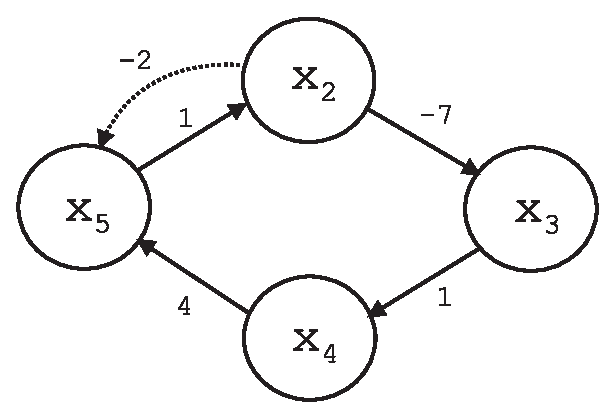
\includegraphics[height=2.0in]{s_iop0/cont01.eps}
\caption{Contradiction Among 4 Atomic Contraints}
\label{fig:siop0:sirn0:scac0:00}
\end{figure}

In Figure \ref{fig:siop0:sirn0:scac0:00},
note that 
(\ref{eq:siop0:sirn0:scac0:05}),
(\ref{eq:siop0:sirn0:scac0:06}),
and (\ref{eq:siop0:sirn0:scac0:07})
imply that $x_5 - x_2 < -2$ (shown with 
a dashed line in the figure), which contradicts
(\ref{eq:siop0:sirn0:scac0:08}).
It is straightforward to see that \emph{any} negative-weight
cycle in a graph of constraints will lead to a contradiction.

We should make formal how 
$\{ <, > \}$ versus $\{ \leq , \geq \}$ are to be treated for
detecting contradictions.  If \emph{all} constraints in the 
cycle involve $\leq$ rather than $<$, then a zero-weight cycle 
does not lead to a contradiction, and a strictly negative-weight
cycle is required to cause a contradiction.  On the other hand,
if at least one constraint in the cycle involves $<$, then both
zero-weight and negative-weight cycles lead to a contradiction.


%%%%%%%%%%%%%%%%%%%%%%%%%%%%%%%%%%%%%%%%%%%%%%%%%%%%%%%%%%%%%%%%%%%%%%%%%%%%%%%
%%%%%%%%%%%%%%%%%%%%%%%%%%%%%%%%%%%%%%%%%%%%%%%%%%%%%%%%%%%%%%%%%%%%%%%%%%%%%%%
%%%%%%%%%%%%%%%%%%%%%%%%%%%%%%%%%%%%%%%%%%%%%%%%%%%%%%%%%%%%%%%%%%%%%%%%%%%%%%%
\subsubsection{Canonical Form Of A Set Of Conjuncted Atomic Constraints}
%Subsection Tag: CFS0
\label{siop0:sirn0:scfs0}

The first question to address is how to assure a canonical
form of a set of atomic constraints (conjuncted together), each in the form
of (\ref{eq:siop0:sirn0:01}).  These results are well
established.  A very compact presentation of these ideas
is given in \cite[pp. 38-44]{bib:p:thsu2k:kglppet}.
Without a guaranteed unique canonical form, certain operations
become impossible; most notably comparison.


%%%%%%%%%%%%%%%%%%%%%%%%%%%%%%%%%%%%%%%%%%%%%%%%%%%%%%%%%%%%%%%%%%%%%%%%%%%%%%%
%%%%%%%%%%%%%%%%%%%%%%%%%%%%%%%%%%%%%%%%%%%%%%%%%%%%%%%%%%%%%%%%%%%%%%%%%%%%%%%
%%%%%%%%%%%%%%%%%%%%%%%%%%%%%%%%%%%%%%%%%%%%%%%%%%%%%%%%%%%%%%%%%%%%%%%%%%%%%%%
\paragraph{Reduction Of Constraints With Same Clocks But Different 
           Constants \mbox{\boldmath $d_{ij}$}:}

It is clear that if there are two [or more] constraints
naming the same variables in the same order with one constraint
tighter than the other, the ``looser'' constraint can be discarded.
For example, consider the two constraints in
(\ref{eq:siop0:sirn0:scfs0:01}) and (\ref{eq:siop0:sirn0:scfs0:02}).
It is clear that (\ref{eq:siop0:sirn0:scfs0:02}) may be discarded,
since (\ref{eq:siop0:sirn0:scfs0:01}) implies
(\ref{eq:siop0:sirn0:scfs0:02}).

\begin{eqnarray}
\label{eq:siop0:sirn0:scfs0:01} 
   x_2 - x_1 & \leq & 3 \\
\label{eq:siop0:sirn0:scfs0:02}
   x_2 - x_1 & \leq & 4
\end{eqnarray}

Similarly, given the two constraints 
(\ref{eq:siop0:sirn0:scfs0:03}) and 
(\ref{eq:siop0:sirn0:scfs0:04}), it is clear that
(\ref{eq:siop0:sirn0:scfs0:04}) can be discarded,
since (\ref{eq:siop0:sirn0:scfs0:03}) implies
(\ref{eq:siop0:sirn0:scfs0:04}).

\begin{eqnarray}
\label{eq:siop0:sirn0:scfs0:03} 
   x_2 - x_1 & < & 4 \\
\label{eq:siop0:sirn0:scfs0:04}
   x_2 - x_1 & \leq & 4
\end{eqnarray}


%%%%%%%%%%%%%%%%%%%%%%%%%%%%%%%%%%%%%%%%%%%%%%%%%%%%%%%%%%%%%%%%%%%%%%%%%%%%%%%
%%%%%%%%%%%%%%%%%%%%%%%%%%%%%%%%%%%%%%%%%%%%%%%%%%%%%%%%%%%%%%%%%%%%%%%%%%%%%%%
%%%%%%%%%%%%%%%%%%%%%%%%%%%%%%%%%%%%%%%%%%%%%%%%%%%%%%%%%%%%%%%%%%%%%%%%%%%%%%%
\paragraph{Reduction Of Contradictory Constraints Implying The Empty Set:}

Constraints can be specified which are contradictory.  Any subset
of contradictory constraints implies that the empty set is specified;
and that all constraints should be discarded and the 
\texttt{is\_empty} flag should be set (the canonical form of the 
empty set).

Section \ref{siop0:sirn0:scac0} has indicated that a necessary 
and sufficient
test for contradictory constraints is a negative-sum or non-positive-sum cycle 
(depending on whether the inequalities involve $\leq$ or $<$) in
the weighted directed graph corresponding to the set of constraints.


%%%%%%%%%%%%%%%%%%%%%%%%%%%%%%%%%%%%%%%%%%%%%%%%%%%%%%%%%%%%%%%%%%%%%%%%%%%%%%%
%%%%%%%%%%%%%%%%%%%%%%%%%%%%%%%%%%%%%%%%%%%%%%%%%%%%%%%%%%%%%%%%%%%%%%%%%%%%%%%
%%%%%%%%%%%%%%%%%%%%%%%%%%%%%%%%%%%%%%%%%%%%%%%%%%%%%%%%%%%%%%%%%%%%%%%%%%%%%%%
\paragraph{Atomic Constraints Involving Different Clocks:}

The final issue to consider in canonical forms is the nature of 
implications---under what circumstances can constraints be removed
because they are implied by other constraints?

In general (\cite[p. 288]{bib:b:modelchecking:clark1999}), 
the implications given in 
(\ref{eq:siop0:sirn0:siac0:01})
through 
(\ref{eq:siop0:sirn0:siac0:04})
hold.

Consider the system of constraints given by
(\ref{eq:siop0:sirn0:scfs0:25}) through 
(\ref{eq:siop0:sirn0:scfs0:27}).  Note that 
(\ref{eq:siop0:sirn0:scfs0:25}) $\wedge$ (\ref{eq:siop0:sirn0:scfs0:26})
$\Longrightarrow$ (\ref{eq:siop0:sirn0:scfs0:27}), so that 
(\ref{eq:siop0:sirn0:scfs0:27}) can be removed from the system
with no effect.

\begin{eqnarray}
\label{eq:siop0:sirn0:scfs0:25} 
   x_3 - x_2 & \leq & 7     \\
\label{eq:siop0:sirn0:scfs0:26}
   x_2 - x_1 & \leq & 3     \\
\label{eq:siop0:sirn0:scfs0:27}
   x_3 - x_1 & \leq & 10  
\end{eqnarray}

Note also that the implication chain resulting in the removal of 
constraints can be more indirect and involve more than three
constraints.  In 
(\ref{eq:siop0:sirn0:scfs0:28}) through 
(\ref{eq:siop0:sirn0:scfs0:31}) note that 
(\ref{eq:siop0:sirn0:scfs0:31}) can be discarded.

\begin{eqnarray}
\label{eq:siop0:sirn0:scfs0:28} 
   x_4 - x_3 & \leq & 7     \\
\label{eq:siop0:sirn0:scfs0:29}
   x_3 - x_2 & \leq & 3     \\
\label{eq:siop0:sirn0:scfs0:30}
   x_2 - x_1 & \leq & 3     \\
\label{eq:siop0:sirn0:scfs0:31}
   x_4 - x_1 & \leq & 14 
\end{eqnarray}

\cite{bib:b:modelchecking:clark1999} phrases 
this problem in terms of \index{shortest path closure}shortest 
path closure of a graph.
In general if there is a ``shorter'' directed path from variable to
variable than the one represented by a constraint, the constraint
is superfluous and
can be removed.  Thus, the implication problem can be
rephrased as a graph theory problem.

As before, some attention must be paid to the distinction between
$\{<, >\}$ and $\{ \leq, \geq \}$.  A constraint 
which represents an ``equal'' path may \index{corner-shaving@``corner-shaving''}
``shave a corner'' of
a region.  Consider the system given by 
(\ref{eq:siop0:sirn0:scfs0:32}) through
(\ref{eq:siop0:sirn0:scfs0:34}).  In this system,
(\ref{eq:siop0:sirn0:scfs0:34}) cannot be discarded without
including the point $(x_1=1, x_2=4)$ in the region,
which would change the region represented.

\begin{eqnarray}
\label{eq:siop0:sirn0:scfs0:32} 
   x_1       & \leq & 4     \\
\label{eq:siop0:sirn0:scfs0:33}
   x_2       & \geq & 1     \\
\label{eq:siop0:sirn0:scfs0:34}
   x_1 - x_2 & <    & 3 
\end{eqnarray}

Following the standard convention that
$x_0 \equiv 0$, (\ref{eq:siop0:sirn0:scfs0:32}) through
(\ref{eq:siop0:sirn0:scfs0:34}) can be rearranged into
the more standard form of (\ref{eq:siop0:sirn0:01}), 
and this more standard
form is given as
(\ref{eq:siop0:sirn0:scfs0:35}) through 
(\ref{eq:siop0:sirn0:scfs0:37}).  This standard form has the
weighted directed graph representation given by
Figure \ref{fig:siop0:sirn0:scfs0:02}.  A few paragraphs
earlier we made the statement that a constraint can be deleted
if a shorter or equivalent length path exists.  However, apparently
we must say in a case such as Figure \ref{fig:siop0:sirn0:scfs0:02} 
that the path $x_2 \rightarrow x_0 \rightarrow x_1$ is
``longer'' than the path $x_2 \rightarrow x_1$, and we must
treat $\{ \leq, \geq \}$ as ``longer'' 
than $\{<, >\}$ for purposes of deciding which constraints can
be removed.  It should also be clear that there are two categories
of path---those that consist exclusively of $\{ \leq, \geq \}$,
and those that do not.  Phrased differently, only one occurrence of
$\{<, >\}$ is required to create the shorter variety of path.

\begin{eqnarray}
\label{eq:siop0:sirn0:scfs0:35} 
   x_1 - x_0 & \leq & 4     \\
\label{eq:siop0:sirn0:scfs0:36}
   x_0 - x_2 & \leq & -1     \\
\label{eq:siop0:sirn0:scfs0:37}
   x_1 - x_2 & <    & 3 
\end{eqnarray}

\begin{figure}
\centering
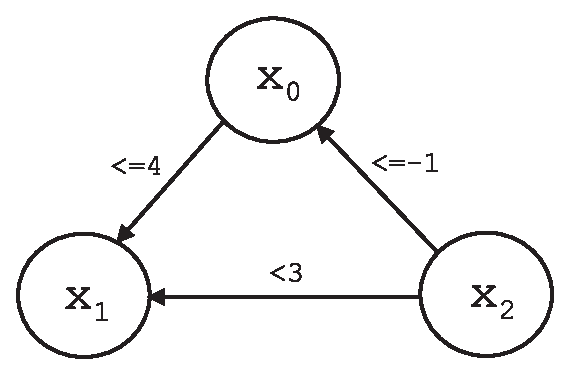
\includegraphics[height=2.0in]{s_iop0/leqeq01.eps}
\caption{``Corner-Shaving'' Of Region}
\label{fig:siop0:sirn0:scfs0:02}
\end{figure}

One question that comes to mind with ``corner-shaving'' is whether
in higher dimensional cases there may be more than one way to 
shave a corner.  It appears that there is not, but again, a proof
is beyond me (Dave Ashley) at this time.

%%%%%%%%%%%%%%%%%%%%%%%%%%%%%%%%%%%%%%%%%%%%%%%%%%%%%%%%%%%%%%%%%%%%%%%%%%%%%%%
%%%%%%%%%%%%%%%%%%%%%%%%%%%%%%%%%%%%%%%%%%%%%%%%%%%%%%%%%%%%%%%%%%%%%%%%%%%%%%%
%%%%%%%%%%%%%%%%%%%%%%%%%%%%%%%%%%%%%%%%%%%%%%%%%%%%%%%%%%%%%%%%%%%%%%%%%%%%%%%
\paragraph{Summary:}

It is believed that the following steps are adequate to ensure a canonical 
form of a conjunction of constraints of the form of
(\ref{eq:siop0:sirn0:01}):

\begin{enumerate}
\item If any cycle with a negative sum of weights appears in the constraints,
      the set is empty and the data structure should be marked to the
      canonical form for the empty set.
\item For constraints involving differences of the same clocks but with different 
      integer constant bounds, the looser constraints can always be removed.
\item Any constraints that do not represent the shortest path between variables
      can be removed.
\end{enumerate}

Again, I (Dave Ashley) am taking some of these approaches on faith for now.
A proof or two would help to reassure my fears.


%%%%%%%%%%%%%%%%%%%%%%%%%%%%%%%%%%%%%%%%%%%%%%%%%%%%%%%%%%%%%%%%%%%%%%%%%%%%%%%
%%%%%%%%%%%%%%%%%%%%%%%%%%%%%%%%%%%%%%%%%%%%%%%%%%%%%%%%%%%%%%%%%%%%%%%%%%%%%%%
%%%%%%%%%%%%%%%%%%%%%%%%%%%%%%%%%%%%%%%%%%%%%%%%%%%%%%%%%%%%%%%%%%%%%%%%%%%%%%%
\subsubsection{Inclusion}
%Subsection Tag: CFS0
\label{siop0:sirn0:sinc0}

To determine if a $A \subseteq B$ for two convex regions
$A$ and $B$, we can note that

\begin{equation}
\label{eq:siop0:sirn0:sinc0:00} 
(A \subseteq B) 
\Longleftrightarrow
(x \in A \rightarrow x \in B)
\Longleftrightarrow
(x \notin B \rightarrow x \notin A) .
\end{equation}

\noindent{}Thus, for every constraint in $B$, there must be
a constraint in $A$ (either directly stated or implied)
which is at least as strong.  This immediately suggests
an algorithm for determining if $A \subseteq B$, which is
provided as Figure \ref{fig:siop0:sirn0:sinc0:00}.

\begin{figure}
\begin{small}
\textbf{Input:} \\
\hspace*{0.15in}$A$ and $B$, two convex regions. \\
\textbf{Output:} \\
\hspace*{0.15in} \emph{TRUE} if $A \subseteq B$, \emph{FALSE} otherwise.\\
\textbf{begin} \\
\hspace*{0.15in}Determine if $A = \O$. \\
\hspace*{0.15in}Determine if $B = \O$. \\
\hspace*{0.15in}\textbf{if} $A = \O$ \textbf{then} return ``\emph{TRUE}''. \\
\hspace*{0.15in}\textbf{for} each constraint in $B$ \\
\hspace*{0.30in}\textbf{begin} \\
\hspace*{0.45in}\textbf{if} constraint involving same clocks exists in $A$ and is at least as tight \\
\hspace*{0.60in}\textbf{then} break (i.e. proceed to next iteration of loop)\\
\hspace*{0.45in}\textbf{elseif} shortest-path closure in $A$ can be found which is at least as tight \\
\hspace*{0.60in}\textbf{then} break \\
\hspace*{0.45in}\textbf{else} \\
\hspace*{0.60in}return ``\emph{FALSE}'' \\
\hspace*{0.30in}\textbf{end} \\
\hspace*{0.15in}return ``\emph{TRUE}'' \\
\textbf{end}
\end{small}
\caption{Algorithm For Determining Inclusion ($A \subseteq B$?)}
\label{fig:siop0:sirn0:sinc0:00}
\end{figure}

Note that it is not necessary for the constraints to
be in a strict canonical
form in order to apply the algorithm shown 
in Figure \ref{fig:siop0:sirn0:sinc0:00}.  However, it is necessary
to rule out $A, B = \O$.\footnote{Need to revisit this later---may not
actually be necessary.}


%%%%%%%%%%%%%%%%%%%%%%%%%%%%%%%%%%%%%%%%%%%%%%%%%%%%%%%%%%%%%%%%%%%%%%%%%%%%%%%
%%%%%%%%%%%%%%%%%%%%%%%%%%%%%%%%%%%%%%%%%%%%%%%%%%%%%%%%%%%%%%%%%%%%%%%%%%%%%%%
%%%%%%%%%%%%%%%%%%%%%%%%%%%%%%%%%%%%%%%%%%%%%%%%%%%%%%%%%%%%%%%%%%%%%%%%%%%%%%%
\subsubsection{Equality}
%Subsubsection Tag: EQU0
\label{siop0:sirn0:sequ0}

There are two possible algorithms for determining equality:

\begin{itemize}
\item A direct algorithm.
\item Defining equality with respect to inclusion, i.e.
      $(A \subseteq B) \wedge (B \subseteq A) \Longrightarrow (A = B)$.
\end{itemize}

For simplicity, we define equality in terms of inclusion (the second
approach above).


%%%%%%%%%%%%%%%%%%%%%%%%%%%%%%%%%%%%%%%%%%%%%%%%%%%%%%%%%%%%%%%%%%%%%%%%%%%%%%%
%%%%%%%%%%%%%%%%%%%%%%%%%%%%%%%%%%%%%%%%%%%%%%%%%%%%%%%%%%%%%%%%%%%%%%%%%%%%%%%
%%%%%%%%%%%%%%%%%%%%%%%%%%%%%%%%%%%%%%%%%%%%%%%%%%%%%%%%%%%%%%%%%%%%%%%%%%%%%%%
\subsection[Implementation Of Unions Of Convex Regions Of $\mathbb{R}^N$]
           {Implementation Of Unions Of Convex Regions Of \mbox{\boldmath $\mathbb{R}^N$}}
%Subsection Tag: URN0
\label{siop0:surn0}

Generally, if a CHM contains only a single path with no branches or loops,
the symbolic state in which the clocks may be at each location is a convex
region of $\mathbb{R}^N$.  This statement is true because the system starts 
at a known unique initial state (a point in $\mathbb{R}^N$, which is 
by definition convex), and each 
operation inherent in carrying the symbolic state through the single path
preserves the convexity.

However, when a CHM contains a cycle or multiple paths leading to a location,
the symbolic state can be a union of convex regions.  Such unions are 
treated as simple arrays of convex regions, and operations on such unions
are defined recursively in terms of the operations on convex regions.

The proposed form for representing a union of convex zones is an unordered array of
convex zones.  The difficulty in dealing with such unions is the difficulty of 
ensuring canonical forms.  This needs to be studied more deeply.


%%%%%%%%%%%%%%%%%%%%%%%%%%%%%%%%%%%%%%%%%%%%%%%%%%%%%%%%%%%%%%%%%%%%%%%%%%%%%%%
%%%%%%%%%%%%%%%%%%%%%%%%%%%%%%%%%%%%%%%%%%%%%%%%%%%%%%%%%%%%%%%%%%%%%%%%%%%%%%%
%%%%%%%%%%%%%%%%%%%%%%%%%%%%%%%%%%%%%%%%%%%%%%%%%%%%%%%%%%%%%%%%%%%%%%%%%%%%%%%
\subsubsection[Canonical Form Of A Union Of Convex Regions Of $\mathbb{R}^N$]
              {Canonical Form Of A Union Of Convex Regions Of \mbox{\boldmath $\mathbb{R}^N$}}
%Subsubsection Tag: CFU0
\label{siop0:surn0:cfu0}

Clearly, there are issues with canonical forms that need to be resolved
when unions are involved.

In particular, forming the union of multiple convex zones can lead to a number of outcomes,
and I'm not sure how to deal with all of those.  Here are the outcomes:

\begin{itemize}
\item The convex zones might not overlap at all.  In this case, 
      it would be guaranteed that taking the canonical form of
      each convex zone, combined with sorting the convex zones somehow,
      would lead to a canonical form.
\item One convex zone may be included in another.  There would be a straightforward
      test for this.  The included zone can be discarded.
\item One convex zone may overlap with another without a subset relationship.  
      In this case there are three outcomes.
      \begin{itemize}
      \item The two convex zones may have a union which forms a larger
            convex zone (for example, one can construct two rectangles
            which overlap in this way).  In this case the two zones can be
            combined.
      \item The two zones may overlap but their union may not be a 
            convex zone.  It may not be possible to adjust either zone
            without changing the region described.
      \item The two zones may overlap, and it may be possible to 
            adjust the zones without changing the region described.
            This immediately leads to concerns about uniqueness of 
            representation and canonical form.
      \end{itemize}
\end{itemize}

Note that some convex regions can be combined with other convex regions
to form another convex region.  For example, rectangles can be combined.

It is \emph{suspected} that the following procedure will result in a canonical
form:

\begin{itemize}
\item Arrange all convex regions in canonical form if necessary
      for subsequent algorithms.

\item Discard any empty sets.

\item Combine any two convex regions that result in any third
      convex region until no such regions can be combined
      any further.  This process would necessarily involve
      discarding inclusions.  (What is the algorithm for this?)

\item For any convex zones with overlap, adjust them downward
      in size as far as possible while not affecting the total
      region described.

\item Arrange convex regions in canonical form if necessary.

\item Sort the convex regions by some sort criteria.

\end{itemize}

Need some proofs to say that this is valid.  Need to think on this
further.


%%%%%%%%%%%%%%%%%%%%%%%%%%%%%%%%%%%%%%%%%%%%%%%%%%%%%%%%%%%%%%%%%%%%%%%%%%%%%%%
%%%%%%%%%%%%%%%%%%%%%%%%%%%%%%%%%%%%%%%%%%%%%%%%%%%%%%%%%%%%%%%%%%%%%%%%%%%%%%%
%%%%%%%%%%%%%%%%%%%%%%%%%%%%%%%%%%%%%%%%%%%%%%%%%%%%%%%%%%%%%%%%%%%%%%%%%%%%%%%
\subsection{Remarks On \swname{} Source Code}
%Subsection Tag: RHS0
\label{siop0:srhs0}


%%%%%%%%%%%%%%%%%%%%%%%%%%%%%%%%%%%%%%%%%%%%%%%%%%%%%%%%%%%%%%%%%%%%%%%%%%%%%%%
%%%%%%%%%%%%%%%%%%%%%%%%%%%%%%%%%%%%%%%%%%%%%%%%%%%%%%%%%%%%%%%%%%%%%%%%%%%%%%%
%%%%%%%%%%%%%%%%%%%%%%%%%%%%%%%%%%%%%%%%%%%%%%%%%%%%%%%%%%%%%%%%%%%%%%%%%%%%%%%
\subsubsection{Source And Documentation File Manifest}
%Subsubsection Tag: SDF0
\label{siop0:srhs0:ssdf0}

This section contains a description of every file of
\swname{} and its documentation.  All of the files listed
below are maintained under version control (\index{CVS}CVS).

\begin{enumerate}
\item \index{mf\_lex.c@\texttt{mf\_lex.c}}%
      \texttt{c:$\backslash$swprojsb$\backslash$hyreach$\backslash$mf\_lex.c} \\
      (File mnemonic:  \emph{m}odel \emph{f}ile \emph{lex}ical analysis.)  Contains functions
      which scan the model input file, lexically analyze it, and deliver a 
      complete ordered list of tokens (in dynamic
      memory) representing the contents of the model input file.
\item \index{mf\_lex.h@\texttt{mf\_lex.h}}%
      \texttt{c:$\backslash$swprojsb$\backslash$hyreach$\backslash$mf\_lex.h} \\
      Header file for \texttt{mf\_lex.c}.
\end{enumerate}


%%%%%%%%%%%%%%%%%%%%%%%%%%%%%%%%%%%%%%%%%%%%%%%%%%%%%%%%%%%%%%%%%%%%%%%%%%
\noindent\begin{figure}[!b]
\noindent\rule[-0.25in]{\textwidth}{1pt}
\begin{tiny}
\begin{verbatim}
$RCSfile: s_iop0.tex,v $
$Source: /cvsroot/esrg/sfesrg/esrgpcpj/hyreach/doc/hyreachm/s_iop0/s_iop0.tex,v $
$Revision: 1.11 $
$Author: dtashley $
$Date: 2002/01/29 17:04:00 $
\end{verbatim}
\end{tiny}
\noindent\rule[0.25in]{\textwidth}{1pt}
\end{figure}
%%%%%%%%%%%%%%%%%%%%%%%%%%%%%%%%%%%%%%%%%%%%%%%%%%%%%%%%%%%%%%%%%%%%%%%%%%
%$Log: s_iop0.tex,v $
%Revision 1.11  2002/01/29 17:04:00  dtashley
%Version control info added, and minor edits.
%
%Revision 1.10  2001/12/01 21:29:54  dtashley
%Safety checkin after edits.
%
%Revision 1.9  2001/11/29 20:15:16  dtashley
%Safety checkin after edits.
%
%Revision 1.8  2001/11/28 19:48:58  dtashley
%Edits.
%
%Revision 1.7  2001/11/09 19:38:16  dtashley
%Safety checkin.
%
%Revision 1.6  2001/11/07 19:52:53  dtashley
%Edits.
%
%Revision 1.5  2001/11/01 06:49:08  dtashley
%Nightly safety check in.
%
%Revision 1.4  2001/10/31 04:31:37  dtashley
%Nightly safety checkin.
%
%Revision 1.3  2001/10/25 05:32:40  dtashley
%Evening safety checkin after edits.
%
%Revision 1.2  2001/09/26 04:51:13  dtashley
%Edits.
%
%Revision 1.1  2001/09/26 02:31:14  dtashley
%Initial checkin, and some edits of main TEX file.
%
%End of S_IOP0.TEX.


%SPBD0: Performance Benchmark Data
\clearpage{}
\input{s_pbd0/s_pbd0}

%SECO0: Warning And Error Codes
\clearpage{}
%$Header: /cvsroot/esrg/sfesrg/esrgpcpj/hyreach/doc/hyreachm/s_eco0/s_eco0.tex,v 1.2 2002/01/30 00:51:04 dtashley Exp $
%
\section[Warning And Error Codes]{Warning Codes And Error Codes Produced By \swname{}}
\label{seco0}

\index{warning codes}\index{error codes}This section explains
all of the warning codes and error codes that can be
generated by \swname{}.  Each warning code or error code
produced by \swname{} consists of 5 characters, accompanied by a a text
message.  Warning codes begin with the `\emph{W}' character, and 
error codes begin with the `\emph{E}' character.

\begin{glossaryenum}
\item \index{WIFLI@\texttt{WIFLI}}\textbf{\texttt{WIFLI}} \\
      (Mnemonic:  \emph{i}ll-\emph{f}ormatted \emph{li}ne.)   The end
      of a line was marked with something other than the expected 13-10 2-byte 
      sequence.  The most likely cause for this warning is that a
      file was transferred in binary mode from a Unix system (Unix 
      traditionally uses only a single byte with the value of 10 to
      mark the end of line).

\item \index{EUTSL@\texttt{EUTSL}}\textbf{\texttt{EUTSL}} \\
      (Mnemonic:  \emph{u}n\emph{t}erminated \emph{s}tring \emph{l}iteral.)
      End of line or end of file was reached while a string literal was
      being processed (i.e. there was an opening quote (`\texttt{"}') but
      no corresponding closing quote before the line or file ended).

\end{glossaryenum}

%%%%%%%%%%%%%%%%%%%%%%%%%%%%%%%%%%%%%%%%%%%%%%%%%%%%%%%%%%%%%%%%%%%%%%%%%%
\noindent\begin{figure}[!b]
\noindent\rule[-0.25in]{\textwidth}{1pt}
\begin{tiny}
\begin{verbatim}
$RCSfile: s_eco0.tex,v $
$Source: /cvsroot/esrg/sfesrg/esrgpcpj/hyreach/doc/hyreachm/s_eco0/s_eco0.tex,v $
$Revision: 1.2 $
$Author: dtashley $
$Date: 2002/01/30 00:51:04 $
\end{verbatim}
\end{tiny}
\noindent\rule[0.25in]{\textwidth}{1pt}
\end{figure}
%%%%%%%%%%%%%%%%%%%%%%%%%%%%%%%%%%%%%%%%%%%%%%%%%%%%%%%%%%%%%%%%%%%%%%%%%%
%$Log: s_eco0.tex,v $
%Revision 1.2  2002/01/30 00:51:04  dtashley
%Nightly safety checkin.
%
%Revision 1.1  2002/01/29 23:51:11  dtashley
%Initial checkin.
%
%Revision 1.5  2002/01/29 17:04:00  dtashley
%Version control info added, and minor edits.
%
%Revision 1.4  2001/10/12 22:32:30  dtashley
%Substantial edits.
%
%Revision 1.3  2001/10/10 02:09:07  dtashley
%Edits.
%
%Revision 1.2  2001/09/26 04:51:13  dtashley
%Edits.
%
%Revision 1.1  2001/09/26 02:31:14  dtashley
%Initial checkin, and some edits of main TEX file.
%
%End of S_INV0.TEX.


%SACK0: Acknowledgements
\clearpage{}
%$Header: /cvsroot/esrg/sfesrg/esrgpcpj/hyreach/doc/hyreachm/s_ack0/s_ack0.tex,v 1.4 2002/01/29 18:47:17 dtashley Exp $
%
\section{Acknowledgements}
\label{sack0}

We are very grateful to Michael J. Burke \cite{bib:i:mburke:visteon}
and Joseph P. DeVoe \cite{bib:i:jdevoe:visteon} of Visteon
for allowing us to re-use without obligation research results,
software components, and documentation which were produced as part
of an earlier paid research effort.

We are grateful to Patricia Bouyer \cite{bib:i:patriciabouyer}
for assistance in locating algorithms for convex hull formation and for
the manipulation of convex regions of $\mathbb{R}^N$.

%%%%%%%%%%%%%%%%%%%%%%%%%%%%%%%%%%%%%%%%%%%%%%%%%%%%%%%%%%%%%%%%%%%%%%%%%%
\noindent\begin{figure}[!b]
\noindent\rule[-0.25in]{\textwidth}{1pt}
\begin{tiny}
\begin{verbatim}
$RCSfile: s_ack0.tex,v $
$Source: /cvsroot/esrg/sfesrg/esrgpcpj/hyreach/doc/hyreachm/s_ack0/s_ack0.tex,v $
$Revision: 1.4 $
$Author: dtashley $
$Date: 2002/01/29 18:47:17 $
\end{verbatim}
\end{tiny}
\noindent\rule[0.25in]{\textwidth}{1pt}
\end{figure}
%%%%%%%%%%%%%%%%%%%%%%%%%%%%%%%%%%%%%%%%%%%%%%%%%%%%%%%%%%%%%%%%%%%%%%%%%%
%$Log: s_ack0.tex,v $
%Revision 1.4  2002/01/29 18:47:17  dtashley
%Safety checkin before taking work home.
%
%Revision 1.3  2002/01/29 17:04:00  dtashley
%Version control info added, and minor edits.
%
%Revision 1.2  2001/10/12 22:32:30  dtashley
%Substantial edits.
%
%Revision 1.1  2001/10/12 00:29:21  dtashley
%Initial checkin.
%End of S_ACK0.TEX.


%SGLO0: Glossary Of Terms
\clearpage
%$Header: /cvsroot/esrg/sfesrg/esrgpcpj/hyreach/doc/hyreachm/s_glo0/s_glo0.tex,v 1.4 2002/01/29 17:04:00 dtashley Exp $
%
\section{Glossary Of Terms}
\label{sglo0}

\begin{glossaryenum}
\item \textbf{CHM}\index{CHM} \\
      \emph{C}omposite \emph{h}ybrid \emph{m}achine.  A timed automaton which is
      created by \swname{} by combining the state-spaces of all EHMs supplied as
      input using a well-defined mathematical operation.  In general, each location
      of a CHM corresponds to one location from each EHM.
\item \textbf{configuration}\index{configuration} \\
      See \emph{location}.
\item \textbf{EHM}\index{EHM} \\
      \emph{E}lementary \emph{h}ybrid \emph{m}achine.  A timed automaton supplied
      as input to \swname{}.
\item \textbf{location}\index{location} \\
      The discrete component of an EHM's state.  The state of an EHM is divided into
      two components:
      \begin{itemize}
      \item The discrete state, which is usually shown on a state transition diagram
            as a circle or a rectangle.
      \item The values of clocks which the EHM sets and tests.  These values are
            conceptually continuous, but for machine representation reasons are
            confined to integers.
      \end{itemize}
      The \emph{location} is the disctete state only.
\item \textbf{on-the-fly}\index{on-the-fly} \\
      Creating (dynamically allocating) the locations of a CHM as needed during 
      verification, rather than in
      advance.  For analyzing reachability, creating locations of a CHM before verification
      begins has performance disadvantages for three reasons:
      \begin{itemize}
      \item A large number of CHM locations may not be reachable, and so are not used
            during the verification.  Creating these locations is a wasted motion.
      \item In the event that an illegal location is reachable, in most cases
            creating all CHM locations
            in advance will greatly slow down finding 
            that the illegal location is reachable.  Because a model with illegal
            states reachable usually requires correction, this will slow down the 
            development cycle in which \swname{} is being used.
      \item For models with a very large state space, not all symbolic information for 
            all locations can be 
            kept in memory at one time (and it is not necessary to do so).  For large
            models, it is not
            possible to create all locations in advance.
      \end{itemize}
\end{glossaryenum}

%%%%%%%%%%%%%%%%%%%%%%%%%%%%%%%%%%%%%%%%%%%%%%%%%%%%%%%%%%%%%%%%%%%%%%%%%%
\noindent\begin{figure}[!b]
\noindent\rule[-0.25in]{\textwidth}{1pt}
\begin{tiny}
\begin{verbatim}
$RCSfile: s_glo0.tex,v $
$Source: /cvsroot/esrg/sfesrg/esrgpcpj/hyreach/doc/hyreachm/s_glo0/s_glo0.tex,v $
$Revision: 1.4 $
$Author: dtashley $
$Date: 2002/01/29 17:04:00 $
\end{verbatim}
\end{tiny}
\noindent\rule[0.25in]{\textwidth}{1pt}
\end{figure}
%%%%%%%%%%%%%%%%%%%%%%%%%%%%%%%%%%%%%%%%%%%%%%%%%%%%%%%%%%%%%%%%%%%%%%%%%%
%$Log: s_glo0.tex,v $
%Revision 1.4  2002/01/29 17:04:00  dtashley
%Version control info added, and minor edits.
%
%Revision 1.3  2001/10/31 04:31:37  dtashley
%Nightly safety checkin.
%
%Revision 1.2  2001/10/01 06:08:09  dtashley
%Basic hacks in place for a workable document.
%
%Revision 1.1  2001/09/26 02:31:14  dtashley
%Initial checkin, and some edits of main TEX file.
%
%End of S_GLO0.TEX.


%SGLO0: Glossary Of Symbols And Mathematical Notation
\clearpage
%$Header: /cvsroot/esrg/sfesrg/esrgpcpj/hyreach/doc/hyreachm/s_glm0/s_glm0.tex,v 1.4 2002/01/29 18:47:17 dtashley Exp $
%
\section{Glossary Of Symbols And Mathematical Notation}
\label{sglm0}

\begin{glossaryenum}
\item {\boldmath{}$\mathbb{R}^N$}\index{RN@$\mathbb{R}^N$} \\
      Under construction.
\end{glossaryenum}


%%%%%%%%%%%%%%%%%%%%%%%%%%%%%%%%%%%%%%%%%%%%%%%%%%%%%%%%%%%%%%%%%%%%%%%%%%
\noindent\begin{figure}[!b]
\noindent\rule[-0.25in]{\textwidth}{1pt}
\begin{tiny}
\begin{verbatim}
$RCSfile: s_glm0.tex,v $
$Source: /cvsroot/esrg/sfesrg/esrgpcpj/hyreach/doc/hyreachm/s_glm0/s_glm0.tex,v $
$Revision: 1.4 $
$Author: dtashley $
$Date: 2002/01/29 18:47:17 $
\end{verbatim}
\end{tiny}
\noindent\rule[0.25in]{\textwidth}{1pt}
\end{figure}
%%%%%%%%%%%%%%%%%%%%%%%%%%%%%%%%%%%%%%%%%%%%%%%%%%%%%%%%%%%%%%%%%%%%%%%%%%
%$Log: s_glm0.tex,v $
%Revision 1.4  2002/01/29 18:47:17  dtashley
%Safety checkin before taking work home.
%
%Revision 1.3  2002/01/29 17:04:00  dtashley
%Version control info added, and minor edits.
%
%Revision 1.2  2001/10/31 04:31:37  dtashley
%Nightly safety checkin.
%
%Revision 1.1  2001/10/30 20:47:48  dtashley
%Initial checkin.
%
%End of S_GLM0.TEX.


%SBIB0: Bibliography
\clearpage
\input{s_bib0/s_bib0}

%SIDX0: Index
\clearpage
%$Header: /cvsroot/esrg/sfesrg/esrgpcpj/hyreach/doc/hyreachm/s_idx0/s_idx0.tex,v 1.2 2001/09/26 04:51:13 dtashley Exp $
%

\printindex{}

%$Log: s_idx0.tex,v $
%Revision 1.2  2001/09/26 04:51:13  dtashley
%Edits.
%
%Revision 1.1  2001/09/26 02:31:14  dtashley
%Initial checkin, and some edits of main TEX file.
%
%End of S_BIB0.TEX.


\end{document}

%$Log: hyreachm.tex,v $
%Revision 1.16  2002/01/30 00:51:04  dtashley
%Nightly safety checkin.
%
%Revision 1.15  2002/01/29 17:04:00  dtashley
%Version control info added, and minor edits.
%
%Revision 1.14  2001/10/31 04:31:37  dtashley
%Nightly safety checkin.
%
%Revision 1.13  2001/10/25 05:32:40  dtashley
%Evening safety checkin after edits.
%
%Revision 1.12  2001/10/12 22:32:30  dtashley
%Substantial edits.
%
%Revision 1.11  2001/10/10 02:09:07  dtashley
%Edits.
%
%Revision 1.10  2001/10/04 17:09:21  dtashley
%Test commit to check merging behavior.
%
%Revision 1.9  2001/10/04 07:09:41  dtashley
%Small trial change.
%
%Revision 1.8  2001/10/03 03:18:03  dtashley
%Superfluous comments removed.
%
%Revision 1.7  2001/10/03 03:15:19  dtashley
%Nightly checkin.
%
%Revision 1.6  2001/10/02 21:05:59  flin
%*** empty log message ***
%
%Revision 1.5  2001/10/02 18:40:48  dtashley
%This is a demonstration change.
%
%Revision 1.4  2001/10/01 06:08:09  dtashley
%Basic hacks in place for a workable document.
%
%Revision 1.3  2001/09/26 04:51:13  dtashley
%Edits.
%
%Revision 1.2  2001/09/26 02:31:14  dtashley
%Initial checkin, and some edits of main TEX file.
%
%Revision 1.1  2001/09/25 22:51:49  dtashley
%Initial checkin.
%
%End of HYREACHM.TEX.
